\subsection{Projektstyring}


\subsection{Problemidentifikation}
Af de givne projektoplæg, har vi valgt at fokusere op det trejde projektoplæg (Når hdverdagen rystes), da dette ser ud til at være det mest spændende for os, da det passer ind i vores interesse og vores kompetencer.





\begin{figure}[h]
    \centering
    \fbox{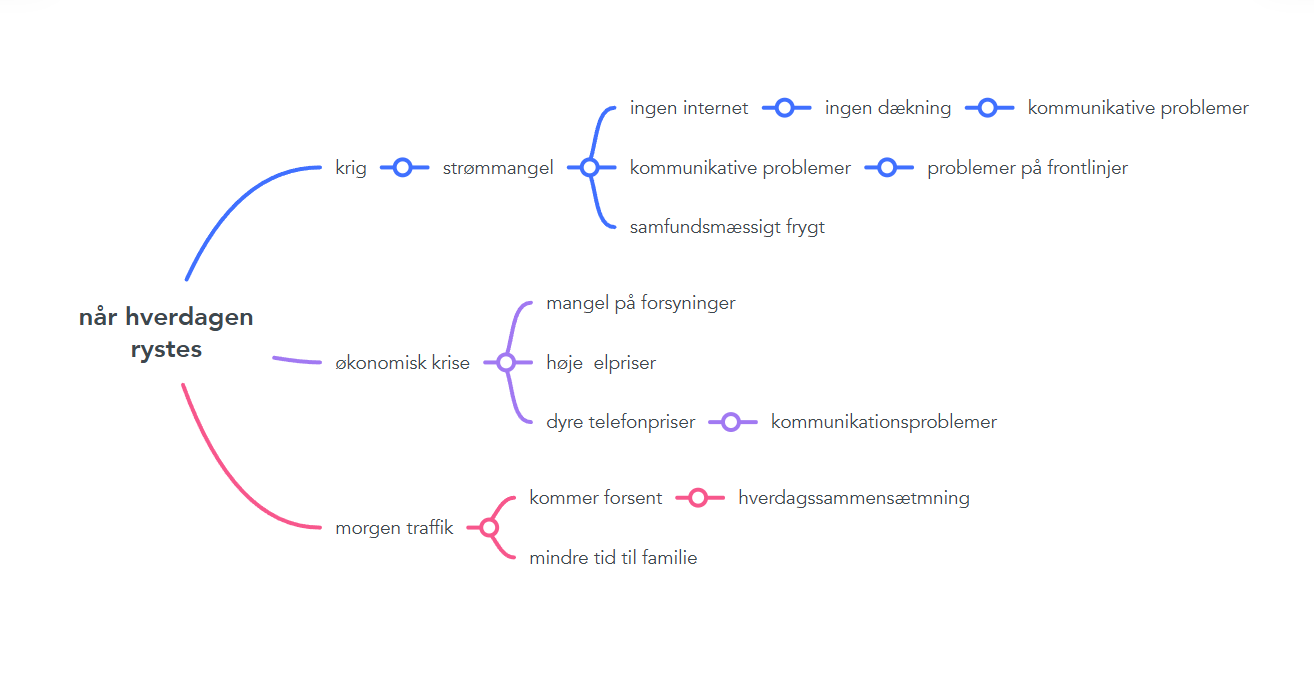
\includegraphics[width=\textwidth]{images/problem-identification.png}}
    \caption{Problemidentifikation}
\end{figure}


I dette projekt, har vi valgt at arbejde med den følgende problemstilling:

Efter ukrainekrigens udbrud i 2022, har verdensbilledet ændret sig markant, det ses bla. ved at beredskabsstyrelsen har lancerert helt kontrete retningslinjer til hvordan danskerne kan forberede sig til eventuelle krisesituationer, som kunne opstå. Hvis en af de krisesituationer, som beskrives i brredsskabssstyrelsens retningslinjer, skulle opstå må det siges at det ville have en stor inflydelse for alle danskernes liv, og heraf vil dette udgør en stor samfundsrelavans.

Vi har i gruppen valgt at opstille et problemtræ, hvilket er en af de teknologifaglige værktøjer, 
som vi kan bruge til at hjælpe med afgrænsningen af det som vi vil arbejde videre med.


\subsection{Afgrænsning}
I denne teknologirapport har vi valgt at afgænse os til at se på hvordan man kan afhjælpe håndteringen af tildkaldelse af nødhjælp, under en krisesituation, hvor mobilnetværket er utilgængeligt.
 